%        File: hw1.tex
%     Created: Sat Apr 06 10:00 AM 2013 P
% Last Change: Sat Apr 06 10:00 AM 2013 P
%
\documentclass[11pt]{article}

\usepackage{amsmath, amssymb, amsthm, cite, graphicx, float, mathrsfs, commath, dsfont, bbm, bm}
\usepackage[mathscr]{eucal}
\usepackage[sc]{mathpazo}
\linespread{1.05}
%\usepackage{setspace}
%\onehalfspacing
\usepackage[margin=1in, top=.8in, left=.8in]{geometry}
\usepackage{color}

% new commands
\DeclareMathOperator*{\argmin}{arg\,min}
\DeclareMathOperator{\sgn}{sgn}
\newcommand{\E}{\mathrm{E}}
\newcommand{\Var}{\mathrm{Var}}
\newcommand{\Cov}{\mathrm{Cov}}
\newcommand{\Cor}{\mathrm{Cor}}
\newcommand{\id}{\operatorname{id}}
\newcommand{\diag}{\operatorname{diag}}
\newcommand{\Id}{\operatorname{Id}}
\newcommand{\tr}{\operatorname{tr}}
\newcommand{\Q}{\mathbb{Q}}
\newcommand{\C}{\mathbb{C}}
\newcommand{\R}{\mathbb{R}}
\newcommand{\Z}{\mathbb{Z}}
\newcommand{\F}{\mathbb{F}}
\newcommand{\N}{\mathbb{N}}

\newcommand{\indep}{\rotatebox[origin=c]{90}{$\models$}}

% 524 commands
%\newcommand{\norm}[1]{\| #1 \|}
\DeclareMathOperator{\spn}{span}
%\newcommand{\spn}{\operatorname{span}}
\newcommand{\onenorm}[1]{\| #1 \|_{L^1(\mathbb R^d)}}
\newcommand{\twonorm}[1]{\| #1 \|_{L^2(\mathbb R^d)}}

% 534 commands
\renewcommand{\Re}{\text{Re\,}}
\renewcommand{\Im}{\text{Im\,}}

\begin{document}
\pagestyle{empty}
\hfill Abraham Engle

\hfill Stat 571

\hfill \today
\begin{enumerate}
    %1
	\item[2.]
		\begin{enumerate}
			%a
			\item Using the notation in the vector outcomes slides, we have $n=30, n_i=2$ for all $i=1,2,\dotsc,n$, $p=4$. For each $i=1,2,\dotsc,n$, I try to fit the model $\bm{Y}_i = \bm{X}_i\beta$, where $\bm{X}_i$ is a 2$\times 4$ covariate matrix for the $i$th leprosy patient. I choose to let 
			\[
				\bm{X}_i = \begin{pmatrix}
			1 & 0 & 0 & 0 \\
			0 & 1 & 1_A & 1_B,
			\end{pmatrix}
			\]
			where $1_A$ is the 0-1 indicator for whether patient $i$ was given antibiotic A and where $1_B$ is similarly defined. This set of matrix equations models for each $i=1,2,\dotsc,n$,
			\begin{align*}
				Y_{i1} &= \beta_0 \\
				Y_{i2} &= \beta_1 + 1_A\beta_2 + 1_B\beta_3,
			\end{align*}
			and if we seek $\widehat{\beta}$ satisfying
			\[
				0 = \frac{1}{n}\sum_{i=1}^n \bm{X}_i^T(\bm{Y}_i - \bm{X}_i\widehat{\beta}),
			\]
			then by construction we have a pair of decoupled plain-vanilla OLS equations for the outcomes $Y_{i1}$ and $Y_{i2}$ since the coefficient $\beta_0$ never appears in the second equation and similarly $\beta_1,\beta_2,\beta_3$ never appear in the first equation. \\ \\
			From this observation, we know $\widehat{\beta}_0 = \frac{1}{n}\sum_{i=1}^n Y_{i1}$ and that $\widehat{\beta}_1$ is a measure of the expected leprosy count among placebo and that $\widehat{\beta}_2$ is an expected deviation from that baseline for those given antibiotic A and $\widehat{\beta}_3$ is an expected deviation from that baseline for those given antibiotic B. From this, we define a transformation $\widehat{\theta} = F(\widehat{\beta})$ via
			\begin{align*}
			\widehat{\theta}_0 &= \widehat{\beta}_0 \\
			\widehat{\theta}_1 &= \frac{\widehat{\beta}_1}{\widehat{\beta}_0} \\
			\widehat{\theta}_2 &= \frac{\widehat{\beta}_1 + \widehat{\beta}_2}{\widehat{\beta}_1} \\
			\widehat{\theta}_3 &= \frac{\widehat{\beta}_1 + \widehat{\beta}_3}{\widehat{\beta}_1}
			\end{align*}
			I am using $\widehat{\beta}_0$ in the denominator of $\widehat{\theta}_1$ instead of the pre-treatment counts of placebo subjects. I spoke with the professor about this slight modification, and I think it is justified since we're assuming no one received any treatment at the beginning of the trial, so the entire population average should be a suitable surrogate for the within-placebo subjects. Obviously this would not be a good thing to use if there was some non-random assignment of treatment groups, but I am also assuming there was sufficient randomization in assigning these groups to justify this.
			%b
			\item I programmed the full set of matrix equations into R and solved them with the multiroot function in the rootSolve package, but as I mentioned in part (a), we could just run two lm's in R, or we could even do both parts by hand. My estimates are
			\begin{align*}
				\widehat{\beta} &= (10.733333, 12.299991, -6.999991, -6.199991)^T \\
				\widehat{\theta} &= (10.7333333,  1.1459619,  0.4308946 , 0.4959353)^T
			\end{align*}
			
			%c
			\item I run $B=10^4$ bootstrap estimates of $\widehat{\beta}$ and produce the following histograms of the parameters:
			\begin{figure}[H]
				\centering
				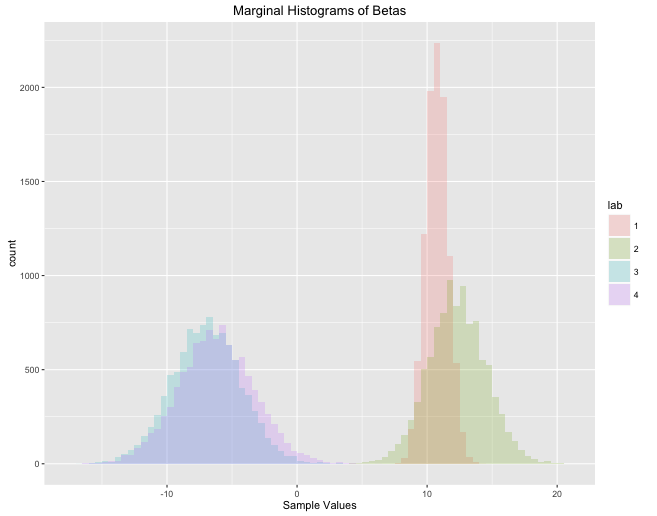
\includegraphics[scale=0.5]{Rplot01}
			\end{figure}
			Bootstrap works on asymptotically normal $\widehat{\beta}$, and the histogram gives me some reassurance for these parameters; however, after transformation, we have (recall $\theta_0 := \beta_0$, so I will not replot the histogram and instead include a QQ plot)
			\begin{figure}[H]
				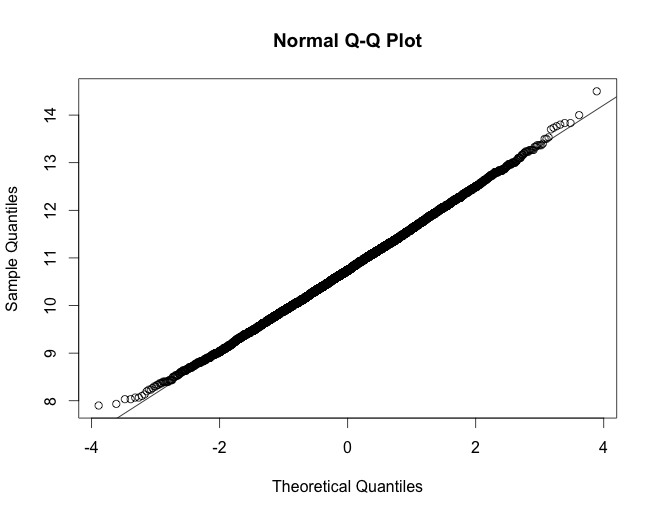
\includegraphics[scale=0.4]{Rplotafter}
				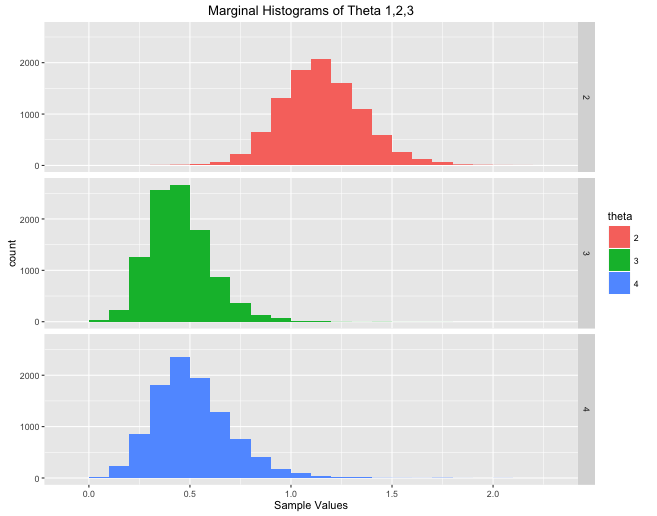
\includegraphics[scale=0.4]{Rplot02}
				\caption{Left Panel: QQ Plot for Bootstrap Distribution of $\widehat{\theta}_0$. Right Panel: Histogram of Bootstrap Samples after Transformation}
			\end{figure}
			To me there is noticeable skewness in the empirical distributions of both $\widehat{\theta}_2$ and $\widehat{\theta}_3$, so I first consider a logarithm transform. Histogram representations of the empirical distributions for $\widehat{\theta}_2$ and $\widehat{\theta}_3$ are 
			\begin{figure}[H]
			\centering			
			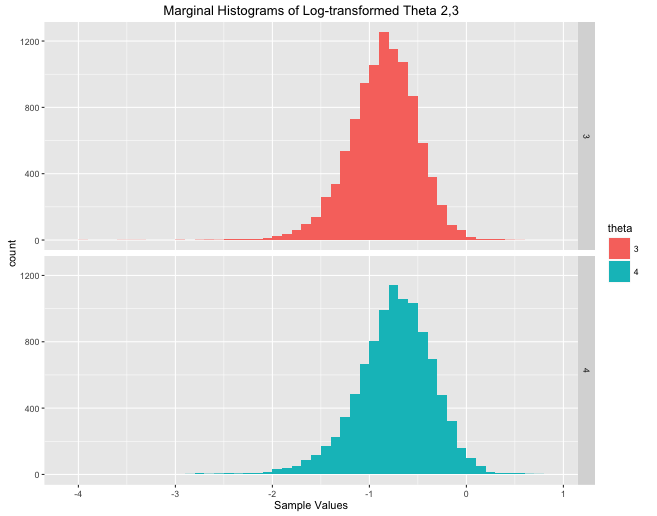
\includegraphics[scale=0.5]{Rplot03}
			\end{figure}
			The QQplots are
			\begin{figure}[H]
				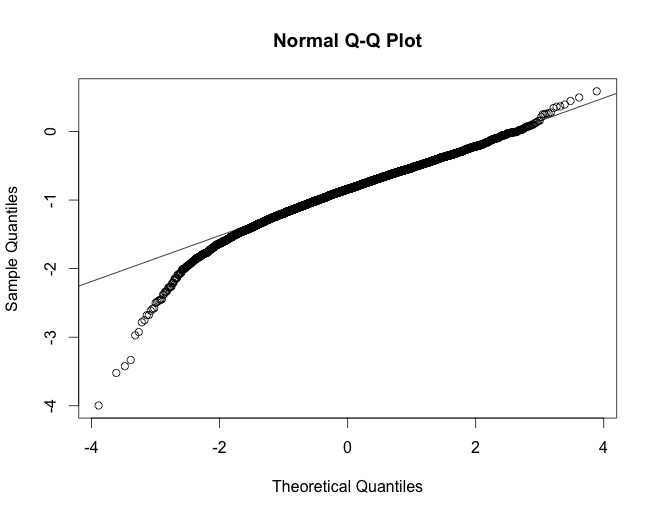
\includegraphics[scale=0.4]{Rplot04}
				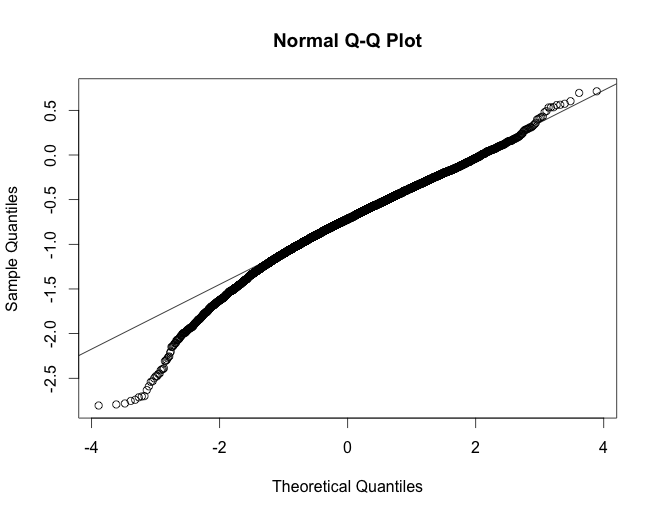
\includegraphics[scale=0.4]{Rplot05}
				\caption{Left Panel: $\widehat{\theta}_2$, Right Panel: $\widehat{\theta}_3$ after Logarithm Transform}
			\end{figure}
			The logarithm did not really help with the heavy tails in my opinion. I will try square root transformations instead:
			\begin{figure}[H]
			\centering
			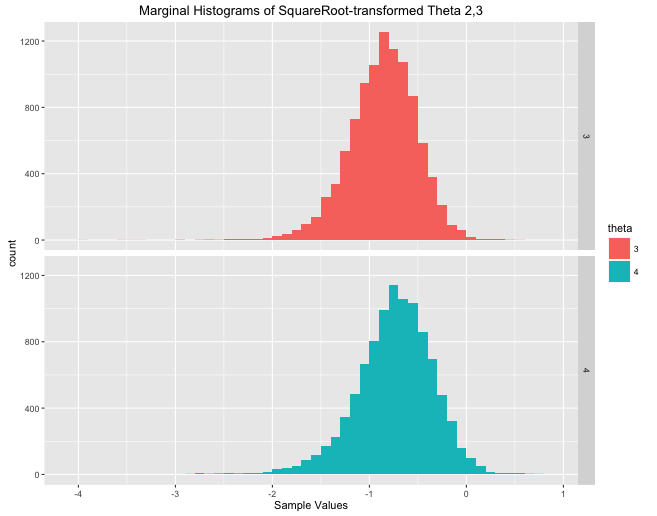
\includegraphics[scale=0.5]{Rplot06}
			\end{figure}
			The QQplots are
			\begin{figure}[H]
				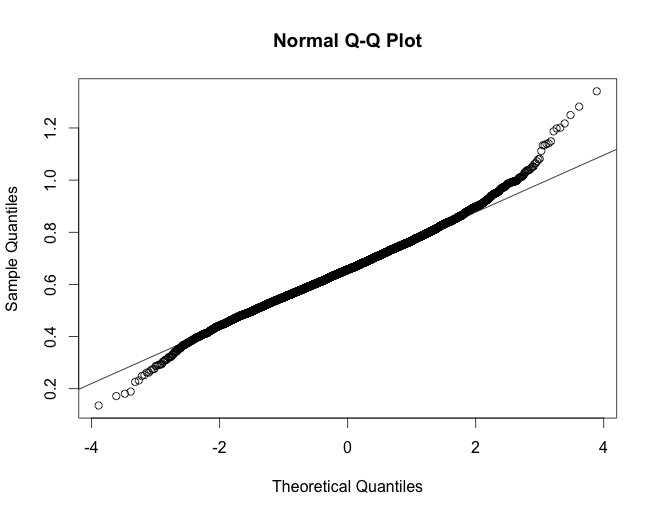
\includegraphics[scale=0.4]{Rplot07}
				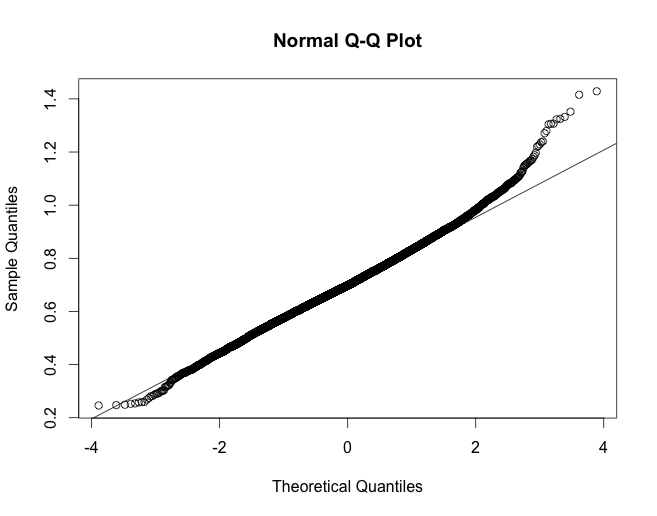
\includegraphics[scale=0.4]{Rplot08}
				\caption{Left Panel: $\widehat{\theta}_2$, Right Panel: $\widehat{\theta}_3$ After Square Root Transform}
			\end{figure}
			I choose to use square root transformations over logarithms and the original definitions. I am still concerned with the relatively heavy tails, but I think the square root provides more symmetry in the distribution. From these empirical distributions, I calculate 95\% confidence intervals as
			\begin{table}[H]
			\centering			
			\begin{tabular}{l||c|c|}
			& Empirical Median & Empirical 95\% CI \\
			\hline
			\hline
			$\theta_0$ & 10.733331&(9.066664, 12.466661)  \\
			\hline
			$\theta_1$ & 1.139416& (0.776699, 1.583046) \\
			\hline
			$\sqrt{\theta_2}$ & 0.6567896& (0.4461230, 0.8930139)\\
			\hline
			$\sqrt{\theta_3}$ & 0.6982549& (0.4478902, 0.9752274) \\
			\end{tabular}
			\caption{Bootstrap Confidence Intervals}
			\end{table}
			%d
			\item From sandwich theory, we know our estimate $\widehat{\beta}$ satisfies
			\[
				\sqrt{n}(\widehat{\beta} - \beta)\to_d N(0_p, A^{-1}BA^{T-1}),
			\]
			and from our new mapping $\widehat{\theta} = G(\widehat{\beta})$ in (c), we apply the $\delta$-method via
			\[
				\sqrt{n}(\widehat{\theta} - \theta) \to_d N(0_p ,J(\beta)A^{-1}BA^{T-1}J(\beta)^T),
			\] 
			and for clarity this $\widehat{\theta}$ has square roots on its third and fourth components. The Jacobian matrix (I used Mathematica and included the notebook at the end of the document) is
			\[
				J(\beta_0,\beta_1,\beta_2,\beta_3) = \begin{pmatrix}
				1 & 0 & 0 & 0 \\
				-\frac{\beta_1}{\beta_0} & \frac{1}{\beta_0} & 0 & 0 \\
				0 & -\frac{\beta_2}{2\beta_1^2\sqrt{\frac{\beta_1+\beta_2}{\beta_1}}} & \frac{1}{2\beta_1\sqrt{\frac{\beta_1+\beta_2}{\beta_1}}} & 0 \\
				0 & -\frac{\beta_3}{2\beta_1^2\sqrt{\frac{\beta_1+\beta_3}{\beta_1}}} & 0 & \frac{1}{2\beta_1\sqrt{\frac{\beta_1+\beta_3}{\beta_1}}}
				\end{pmatrix}
			\]
			From consistency, I evaluate $J$ at $\widehat{\beta}$ and use the estimates in the slides, noting that $g$ is the identity map so that $\nabla_\beta g(\bm{X}_i\beta) = \bm{X}_i$.
			\[
				\widehat{A} = \frac{1}{n} \sum_{i=1}^n \nabla_\beta [\bm{X}_i^T(\bm{Y}_i - \bm{X}_i\beta)]\big|_{\beta=\widehat{\beta}} = -\frac{1}{n} \sum_{i=1}^n \bm{X}_i^T\bm{X}_i
			\]
			and
			\[
				\widehat{B} = \frac{1}{n} \sum_{i=1}^n (\bm{Y}_i - \bm{X}_i\widehat{\beta})(\bm{Y}_i - \bm{X}_i\widehat{\beta})^T.
			\]
			Implementing all this in R, we arrive at the following table:
						\begin{table}[H]
			\centering			
			\begin{tabular}{l||c|c|}
			& EE Value & 95\% Sandwich CI \\
			\hline
			\hline
			$\theta_0$ & 10.733331&(9.047446, 12.419220)  \\
			\hline
			$\theta_1$ & 1.1459619& (0.767877, 1.524047) \\
			\hline
			$\sqrt{\theta_2}$ & 0.6564256& (0.4534951, 0.8593562)\\
			\hline
			$\sqrt{\theta_3}$ & 0.7042268 & (0.4631438, 0.9453097) \\
			\end{tabular}
			\caption{Sandwich Confidence Intervals}
			\end{table}
			There is some loss of interpretation after the square root transform, but I am more comfortable reporting bootstrap intervals afterwards. 
		\end{enumerate}
\end{enumerate}
\newpage
R Code for HW2
\begin{verbatim}
library(rootSolve)
library(ggplot2)
setwd("~/Dropbox/UW2015-2016/Win2016/571/hw2")
setwd("C:/Users/aengl_000/Dropbox/UW2015-2016/Win2016/571/hw2")
lep <- read.table("leprosy.txt", header=TRUE, sep=" ")
#treatment 1 - antibiotic A
#treatment 2 - antibiotic B
#treatment 3 - placebo
#count1: Pre-treatment count of bacilli, at six sites of the body where the bacilli
 tend to congregate
#count2: Post-treatment count of bacilli (lower is better)
#severe: Indicator of severe disease, prior to the trial (0=No, 1=Yes)
attach(lep)
n = dim(lep)[1]
ni = 2 #same for all i
p = 4 #four parameters

X = matrix(0,nrow=60,ncol=4) #sum(ni) x p is 60 x 4 stacked matrix
X[seq(1,59,by=2),] <- rep(c(1,0,0,0),each=30)
X[seq(2,60,by=2),] <- rep(c(0,1,0,0),each=30)
for(i in 1:30)
{
  if(trt[i] == 1)
  {
    X[2*i,3] = 1
  }
  if(trt[i] == 2)
  {
    X[2*i,4] = 1
  }
}

Y = rbind(count1,count2)
est <- function(beta){
  temp = 0
  count = 1
  for(i in seq(1,59,by=2))
  {
    temp = temp + t(X[c(i,i+1),])%*%(t(t(Y[,count]))-X[c(i,i+1),]%*%beta)
    count = count +1
  }
  return(
    (1/n)*temp
  )
}
beta = multiroot(est,start=c(10,0,0,0))$root
theta = c(beta[1],beta[2]/beta[1] ,(beta[2]+beta[3])/beta[2] ,(beta[2]+beta[4])/beta[2])

set.seed(1)
boot <- function(B)
{
  betas <- matrix(0, nrow=B, ncol=4)
  for(b in 1:B)
  {
    ind <- sample(1:30, 30, replace=TRUE)
    tempdat <- lep[ind,]
    X = matrix(0,nrow=60,ncol=4) #sum(ni) x p is 60 x 4 stacked matrix
    X[seq(1,59,by=2),] <- rep(c(1,0,0,0),each=30)
    X[seq(2,60,by=2),] <- rep(c(0,1,0,0),each=30)
    for(i in 1:30)
    {
      if(tempdat$trt[i] == 1)
      {
        X[2*i,3] = 1
      }
      if(tempdat$trt[i] == 2)
      {
        X[2*i,4] = 1
      }
    }
    Y = rbind(tempdat$count1,tempdat$count2)
    est <- function(beta){
      temp = 0
      count = 1
      for(i in seq(1,59,by=2))
      {
        temp = temp + t(X[c(i,i+1),])%*%(t(t(Y[,count]))-X[c(i,i+1),]%*%beta)
        count = count +1
      }
      return(
        (1/n)*temp
      )
    }
    beta = multiroot(est,start=c(0,0,0,0))$root
    betas[b,] <- beta
  }
  return(betas)
}
betas <- boot(10000)
dat = data.frame(bs=c(betas[,1], betas[,2], betas[,3], betas[,4]),
 lab=as.factor(rep(1:4, each=10^4)))

ggplot(dat, aes(x=bs, fill=lab)) +
  geom_histogram(alpha=0.2, position="identity", binwidth=0.5) +
  xlab("Sample Values")+
  ggtitle("Marginal Histograms of Betas")

theta1 <- betas[,1]
theta2 <- betas[,2]/betas[,1]
theta3 <- (betas[,2] + betas[,3])/betas[,2]
theta4 <- (betas[,2] + betas[,4])/betas[,2]

dat2 = data.frame(bs=c(theta2,theta3,theta4), theta=as.factor(rep(2:4, each=10^4)))

ggplot(dat2, aes(x=bs, fill=theta)) +
  geom_histogram(binwidth=0.1) + facet_grid(theta~.)+
  xlab("Sample Values")+
  ggtitle("Marginal Histograms of Theta 2,3,4")


dat3 = data.frame(bs=c(log(theta3),log(theta4)), theta=as.factor(rep(3:4, each=10^4)))
ggplot(dat3, aes(x=bs, fill=theta)) +
  geom_histogram(binwidth=0.1) + facet_grid(theta~.)+
  xlab("Sample Values")+
  ggtitle("Marginal Histograms of Log-transformed Theta 3,4")

qqnorm(log(theta3))
qqline(log(theta3))

qqnorm(log(theta4))
qqline(log(theta4))


dat4 = data.frame(bs=c(sqrt(theta3),sqrt(theta4)), theta=as.factor(rep(3:4, each=10^4)))
ggplot(dat3, aes(x=bs, fill=theta)) +
  geom_histogram(binwidth=0.1) + facet_grid(theta~.)+
  xlab("Sample Values")+
  ggtitle("Marginal Histograms of SquareRoot-transformed Theta 3,4")
qqnorm(sqrt(theta3))
qqline(sqrt(theta3))

qqnorm(sqrt(theta4))
qqline(sqrt(theta4))

CI1 <- quantile(theta1,probs=c(0.025,0.5,0.975))
CI2 <- quantile(theta2,probs=c(0.025,0.5, 0.975))
CI3 <- quantile(sqrt(theta3),probs=c(0.025,0.5,0.975))
CI4 <- quantile(sqrt(theta4),probs=c(0.025,0.5,0.975))
#p2p4
J3 <- function(x)
{
  p = length(x)
  return(
    matrix(c(1,0,0,0,
             -x[2]/x[1]^2,1/x[1],0,0,
             0,-x[3]/(2*x[2]^2*sqrt((x[2]+x[3])/x[2])),1/(2*x[2]*sqrt((x[2]+x[3])/x[2])),0,
             0,-x[4]/(2*x[2]^2*sqrt((x[2]+x[4])/x[2])),0,1/(2*x[2]*sqrt((x[2]+x[4])/x[2]))),
              nrow=p, ncol=p, byrow=TRUE)
  )
}
Bhat = 0
count = 1
for(i in seq(1,59,by=2))
{
  Bhat = Bhat + t(X[c(i,i+1),])%*%(t(t(Y[,count]))-X[c(i,i+1),]%*%beta)
  %*%t(t(X[c(i,i+1),])%*%(t(t(Y[,count]))-X[c(i,i+1),]%*%beta))
  count = count +1
}
Bhat = Bhat/n

Ahat = 0
for(i in seq(1,59,by=2))
{
  Ahat = Ahat - t(X[c(i,i+1),])%*%X[c(i,i+1),]
}
Ahat = Ahat/n

thetanew2 = c(beta[1],beta[2]/beta[1] ,sqrt((beta[2]+beta[3])/beta[2])
 ,sqrt((beta[2]+beta[4])/beta[2]))
sandNEW2 = J3(beta)%*%solve(Ahat)%*%Bhat%*%solve(t(Ahat))%*%t(J3(beta))/n
CIsand1NEW2 <- thetanew2[1] + 1.96*sqrt(sandNEW2[1,1])*c(-1,1)
CIsand2NEW2 <- thetanew2[2] + 1.96*sqrt(sandNEW2[2,2])*c(-1,1)
CIsand3NEW2 <- thetanew2[3] + 1.96*sqrt(sandNEW2[3,3])*c(-1,1)
CIsand4NEW2 <- thetanew2[4] + 1.96*sqrt(sandNEW2[4,4])*c(-1,1)


#before square root transformaiton, not very good...
theta <- c(beta[1],beta[2]/beta[1] ,(beta[2]+beta[3])/beta[2] ,(beta[2]+beta[4])/beta[2])
sand = J(beta)%*%solve(Ahat)%*%Bhat%*%solve(t(Ahat))%*%t(J(beta))/n
CIsand1 <- theta[1] + 1.96*sqrt(sand[1,1])*c(-1,1)
CIsand2 <- theta[2] + 1.96*sqrt(sand[2,2])*c(-1,1)
CIsand3 <- theta[3] + 1.96*sqrt(sand[3,3])*c(-1,1)
CIsand4 <- theta[4] + 1.96*sqrt(sand[4,4])*c(-1,1)

sandt <- solve(Ahat)%*%Bhat%*%solve(t(Ahat))/n


#these below are from untransformed, very good
CIsandt1 <- beta[1] + 1.96*sqrt(sandt[1,1])*c(-1,1)
CIsandt2 <- beta[2] + 1.96*sqrt(sandt[2,2])*c(-1,1)
CIsandt3 <- beta[3] + 1.96*sqrt(sandt[3,3])*c(-1,1)
CIsandt4 <- beta[4] + 1.96*sqrt(sandt[4,4])*c(-1,1)

CIt1 <- quantile(betas[,1],probs=c(0.025,0.975))
CIt2 <- quantile(betas[,2],probs=c(0.025,0.975))
CIt3 <- quantile(betas[,3],probs=c(0.025,0.975))
CIt4 <- quantile(betas[,4],probs=c(0.025,0.975))

####intervals from log transform of parameters
# J2 <- function(x)
# {
#   p = length(x)
#   return(
#     matrix(c(1,0,0,0,
#              -x[2]/x[1]^2,1/x[1],0,0,
#              0,-x[3]/(x[2]^2+x[2]*x[3]),1/(x[2]+x[3]),0,
#              0,-x[4]/(x[2]^2+x[2]*x[4]),0,1/(x[2]+x[4])), nrow=p, ncol=p, byrow=TRUE)
#   )
# }
# thetanew = c(beta[1],beta[2]/beta[1] ,log((beta[2]+beta[3])/beta[2]) ,log((beta[2]+beta[4])/beta[2]))
# sandNEW = J2(beta)%*%solve(Ahat)%*%Bhat%*%solve(t(Ahat))%*%t(J2(beta))/n
# CIsand1NEW <- thetanew[1] + 1.96*sqrt(sandNEW[1,1])*c(-1,1)
# CIsand2NEW <- thetanew[2] + 1.96*sqrt(sandNEW[2,2])*c(-1,1)
# CIsand3NEW <- thetanew[3] + 1.96*sqrt(sandNEW[3,3])*c(-1,1)
# CIsand4NEW <- thetanew[4] + 1.96*sqrt(sandNEW[4,4])*c(-1,1)
# 
# theta1NEW <- betas[,1]
# theta2NEW <- betas[,2]/betas[,1]
# theta3NEW <- log((betas[,2] + betas[,3])/betas[,2])
# theta4NEW <- log((betas[,2] + betas[,4])/betas[,2])
# CI1new <- quantile(theta1NEW,probs=c(0.025,0.975))
# CI2new <- quantile(theta2NEW,probs=c(0.025,0.975))
# CI3new <- quantile(theta3NEW,probs=c(0.025,0.975))
# CI4new <- quantile(theta4NEW,probs=c(0.025,0.975))
\end{verbatim}
Mathematica:
\begin{figure}[H]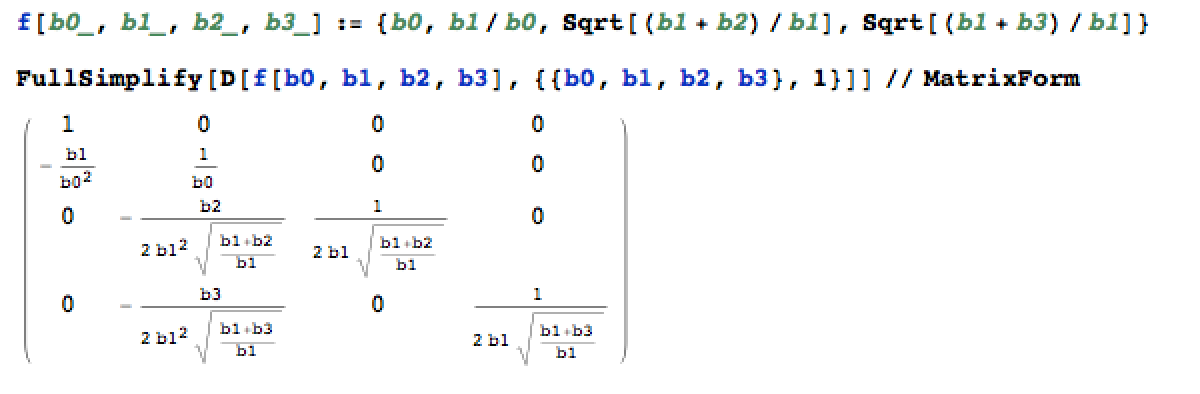
\includegraphics[scale=0.5]{hw2.png}
\end{figure}
\end{document}



